\subsection{Software Implementation Overview} \label{sec:software_overview}
Figure~\ref{fig:code-overview-flowchart} illustrates the overall system architecture and control flow.
\begin{figure}[h]
	\centering
	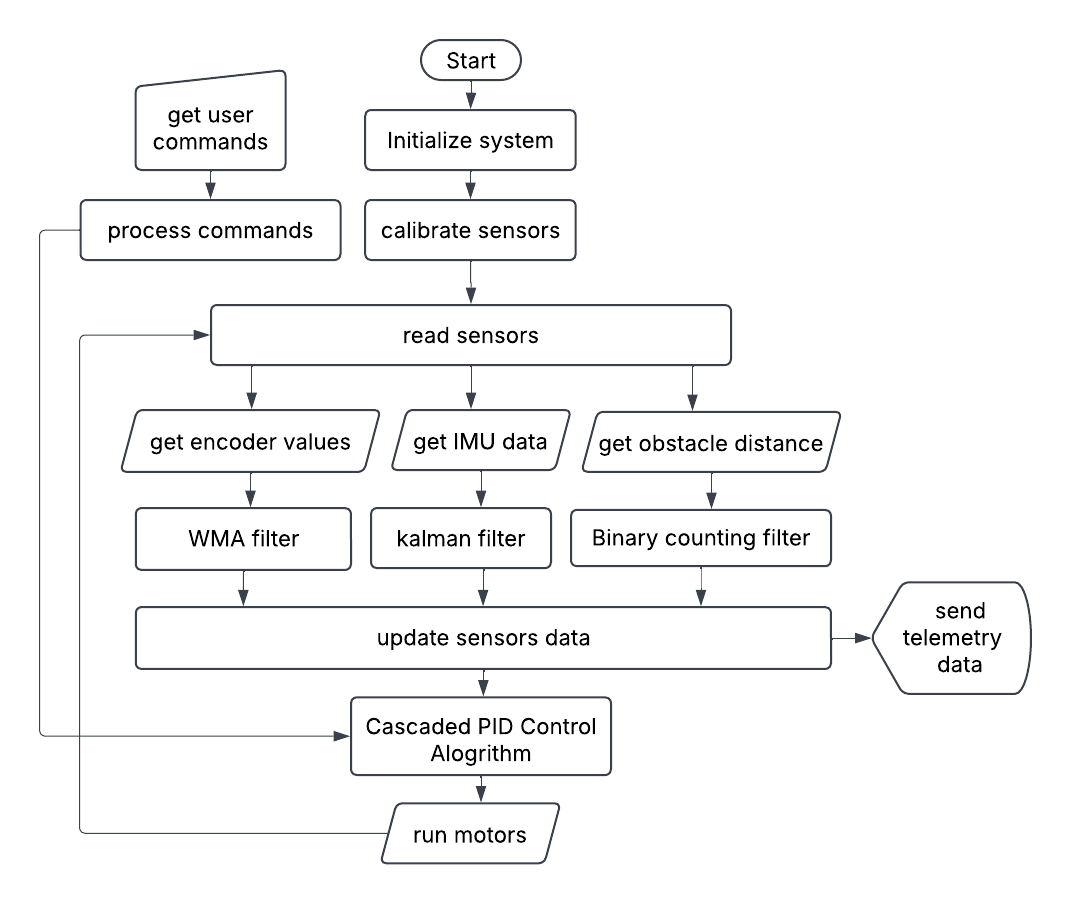
\includegraphics[width=0.8\linewidth]{assets/code_overview_flowchart.png}
	\caption{System operational flowchart.}
	\label{fig:code-overview-flowchart}
\end{figure}

The process begins with the reception of user commands, which are then parsed and processed.  Subsequently, the system initializes and calibrates its various sensors.  Sensor data, including encoder values, IMU data, and obstacle distance, is acquired and passed through respective filters (WMA, Kalman, and Binary Counting) to reduce noise and improve accuracy.  The filtered sensor data is then aggregated and used to update the robot's internal state.

\begin{figure}[h]
	\centering
	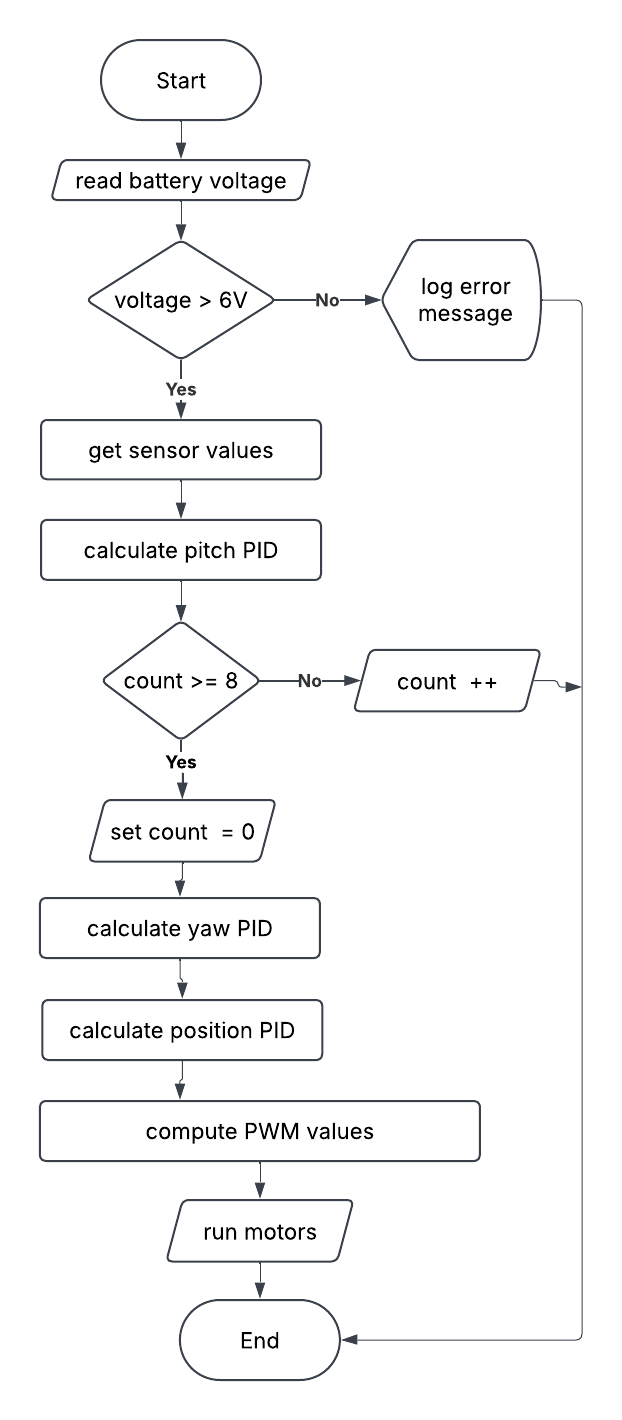
\includegraphics[width=0.5\linewidth]{assets/control_loop_diagram.png}
	\caption{A simplified block diagram of the cascaded control loop used. }
	\label{fig:control-loop}
\end{figure}

To stabilize the inverted pendulum in the upright position and to control the robot at the desired position using the PID control approach, two PID controllers with Linear–quadratic regulator (LQR) control : Yaw angle PID controller and position PID controller have been designed for the two control loops of the system.

A cascaded PID control algorithm (shown in Fig.~\ref{fig:control-loop}) utilizes the updated sensor data to calculate appropriate motor commands. These commands are then sent to the motors, driving the robot's movement.  Throughout this process, telemetry data is generated and transmitted, providing feedback on the robot's status and performance.  This closed-loop control and monitoring system ensures precise and reliable operation. Further details on the individual components and algorithms are provided in the following subsections.